


%%%%%%%%%%
\documentclass[fleqn,reqno,10pt]{article}
\usepackage{graphicx}
\usepackage{multicol}

\usepackage{amsmath}
\usepackage[margin = 2.5cm]{geometry}
\usepackage[natbib=true,style=authoryear-comp,backend=bibtex,doi=false,url=false]{biblatex}
\bibliography{bibliography,biblio}

\usepackage{txfonts} % times font
\usepackage{relsize} % provides command \relsize{+/-x} for relative font size changes

% abbreviations in small-caps
\usepackage{xspace}
\newcommand{\acro}[1]{{\relsize{+1}\textsc{#1}}\xspace}
\newcommand{\acros}[1]{{\relsize{+1}\textsc{#1}}{\relsize{-1}s}\xspace}
\newcommand{\ga}{\acro{ga}}    % gradable adjective
\newcommand{\gas}{\acros{gas}} % gradable adjectives

\newcommand{\den}[1]{\left [\! \left [ #1 \right ]\! \right]}

% colors
\usepackage[dvipsnames]{xcolor}
\definecolor{Red}{RGB}{178,34,34}
\definecolor{Green}{RGB}{34,178,34}
\newcommand{\mf}[1]{\textcolor{Red}{[mf: #1]}}
\newcommand{\bt}[1]{\textcolor{Green}{[lb: #1]}}
\newcommand{\red}[1]{{\color{Red}{#1}}}

% some commands
\newcommand{\set}[1]{\left\{#1\right\}}
\newcommand{\tuple}[1]{\left \langle #1\right\rangle}
\DeclareMathOperator{\expo}{exp}
\DeclareMathOperator*{\argmin}{arg\,min}
\DeclareMathOperator*{\argmax}{arg\,max}


\title{Notes from 1\textsuperscript{st} brainstorming}
\author{Barbara and Michael}
\date{February 8 2018}

\begin{document}
\maketitle

\section{Background: theories and experimental data}
\label{sec:backgr-theor-exper}

\section{Models}

Rather than redo, outwit or refute previous experimental contributions, \textbf{our goal is to
  chart new territory}. The starting point should be new predictions made by conceptually
interesting probabilistic models, ideally extensions of the optimal-$\theta$ model or the RSA
model for \gas
\citep{QingFranke2014:Meaning-and-Use,QingFranke2014:Gradable-Adject,LassiterGoodman2015:Adjectival-vagu}. Two
ideas came to mind.

\subsection{Lexical uncertainty about absolute \gas}

Lexical uncertainty models
\citep{BergenLevy2012:Thats-what-she-,PottsLassiter2016:Embedded-implic,BergenLevy2014:Pragmatic-Reaso}
assume that the listener is uncertain about the lexical meaning that a speaker might bring to
the conversation. We consider uncertainty about the lexical meaning of absolute \gas: do they
receive a relative (prior dependent) or absolute (pure standard) interpretation. We combine
lexical uncertainty with the \ga-model of \citet{LassiterGoodman2015:Adjectival-vagu}
\citep[exactly what][did too]{TesslerFranke2018:Not-unreasonabl}:
\begin{align}
L_{1}(x, \theta, \mathcal{L} \mid u) &\propto S_{1}(u \mid x, \theta, \mathcal{L}) \cdot P(x) \cdot  P(\theta) \cdot P(\mathcal{L}) \label{eq:L1} \\
S_{1}(u \mid x, \theta, \mathcal{L}) &\propto \exp{(\alpha \cdot \ln {L_{0}(x \mid u, \theta, \mathcal{L})} - \text{cost}(u))} \label{eq:S1}\\
L_{0}(x \mid u, \theta, \mathcal{L}) &\propto \mathcal{L}(u, x, \theta) \cdot P(x) \label{eq:L0}
\end{align}
A lexicon is a map $\mathfrak{L} \colon u,x,\theta \mapsto \set{0;1}$ which gives a (Boolean)
truth-value for any utterance $u$ of some \ga, degree $x$ and threshold $\theta$. Only absolute
gradable adjectives are lexically uncertain in the way described above. Model variants could
distinguish cases where speakers maintain a single rule (all absolute \gas are
prior-dependent/pure-standard) or between-item flexibility (e.g., \emph{full} is prior
dependent; \emph{bent} is not).

This model is likely to make interesting \textbf{novel predictions about task effects} that
other stories are unlikely to offer anything beyond hand-wavy explanations. Generally speaking,
observations from previous trials/encounters could shift beliefs about the speaker's likely
lexicon. If speaker's have been observed to use an absolute \ga to refer to non-absolute degree
$x$, listeners should update their lexical beliefs accordingly and be more likely to interpret
a future use of this \ga (or others, depending on the model variant) as relative-standard
(prior-dependent). Also, interpretation tasks which display multiple utterances at the same
time ((implicitly:) by the same speaker) could show interesting effects of jointly conditioning
the model with all observed utterances \citep[as observed
by][]{TesslerFranke2018:Not-unreasonabl}.

\mf{models need to be formulated precisely, implemented and predictions checked; this is all
  just intuitive guesses about potential model predictions}

\subsection{Uncertainty about the prior (or the comparison class)}

If speakers and listeners are uncertain about the prior over degrees $P(x)$, we are also bound
to see potentially interesting \textbf{predictions about response dynamics as a function of
  prior exposure}. Suppose that items to be judged or chosen for interpretation are presented
individually in each trial, or at the same time (like in stuff from the Chicago group \citep{KimXiangKennedy:2014,LeffelXiangKennedy:2016}
\mf{insert ref}), this task manipulation will likely have effects on participants' construction
of the comparison class / the relevant prior distribution. For example, for absolute \gas it
might matter whether the end-point degrees have already been observed or not: as long as there
is uncertainty about how likely these belong to the comparison class, priors with little
density on these degrees are reasonably likely, thus shifting predictions about $\theta$
``further away from the end-points''. In general, the more extreme instances are observed, the
more median instances should count as ``neither this nor that''. 

\subsection{Relevant experimental results}

\citet{KimXiangKennedy:2014} find evidence that absolute, but not relative, adjectives show signs of having context-invariant, precise meanings. In Experiment 1, they find that the thresholds for relative adjectives are sensitive to the local context (grouped vs. isolated presentation in the picture below), but those for absolute adjectives are not. They find a significant effect of scale position for relative adjectives in grouped presentation (but not in isolated presentation); and no difference for absolute adjectives by presentation type. In the judgments for relative adjectives, there was more variance due to noun identity (in isolated presentation). In the judgments for absolute adjectives, there was more variance due to adjective identity (no difference by presentation type).\\
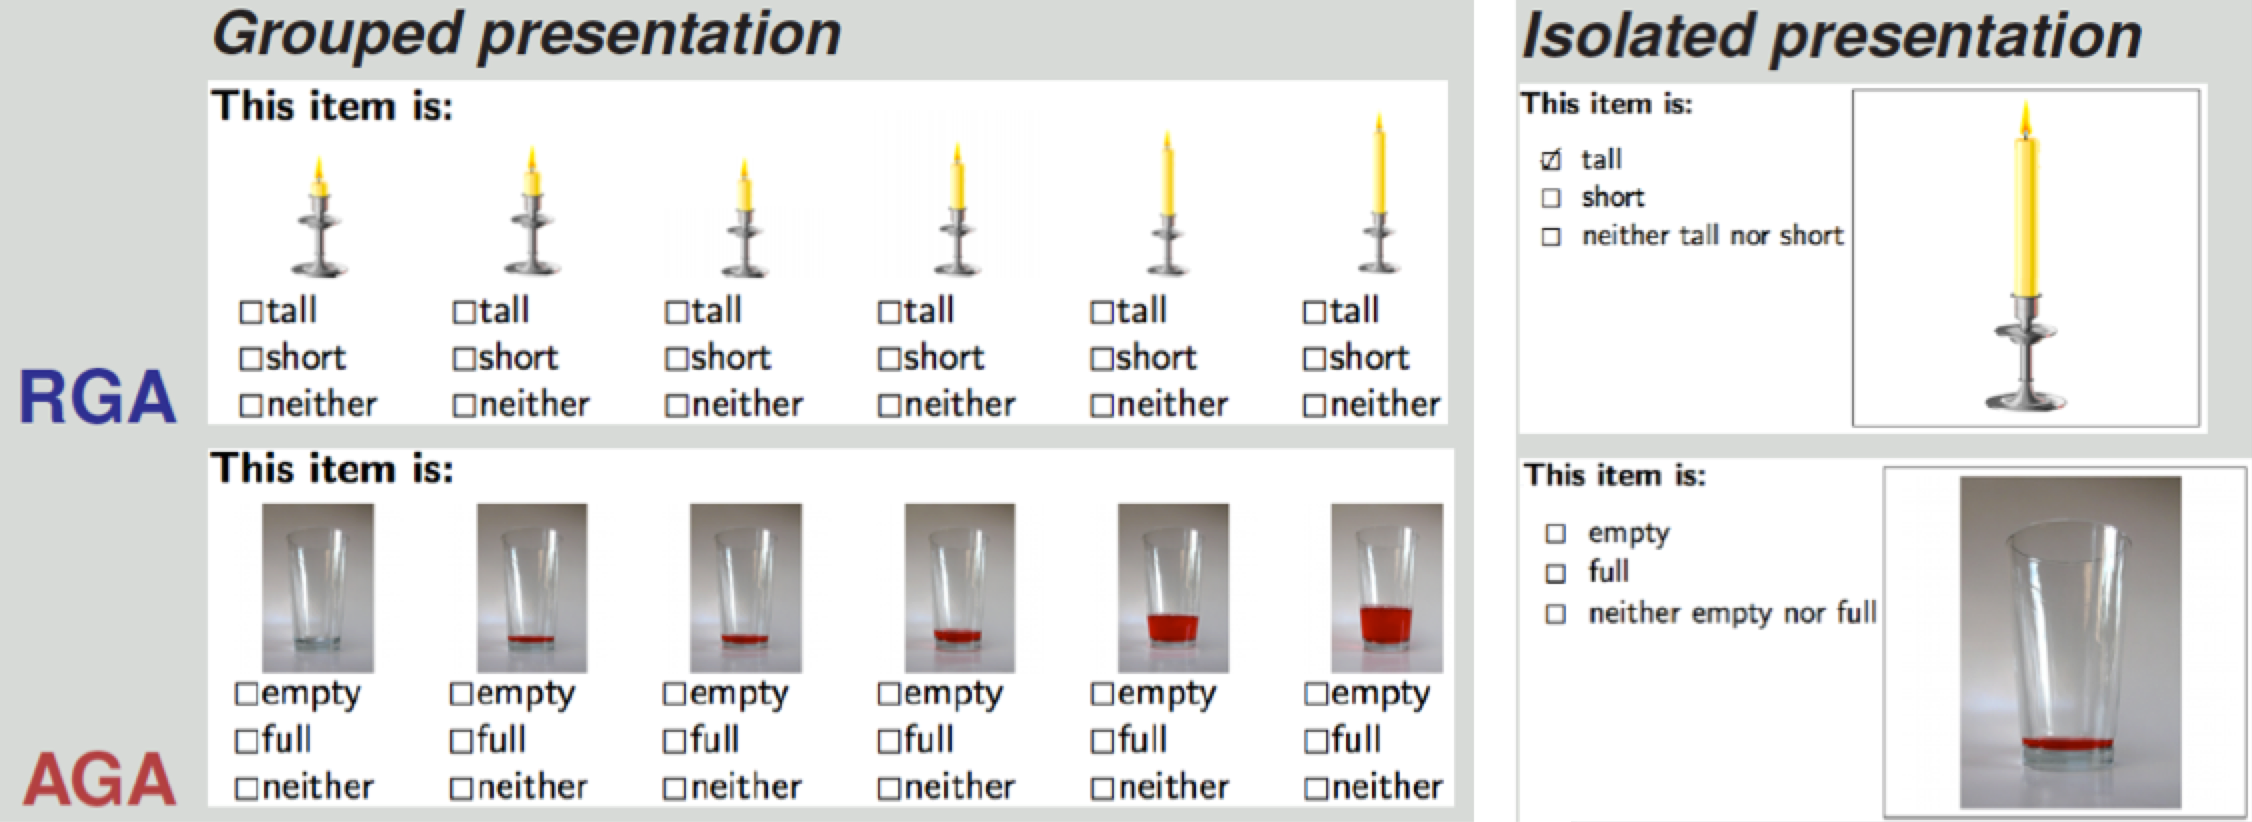
\includegraphics[width=9cm]{images/kim-xiang-kennedy-groups-isolated.png}\\
In Experiment 2 with just isolated presentation, they find that only absolute adjectives show asymmetric shiftability: they allow shifts to higher levels of precision, and resist loosening a standard that was previously set at maximum precision (main effect of previous precise exemplar (i.e. previous exposure to items like the completely empty cup above) and an interaction with scale position, but no interaction with number of intervening uses of the same adjective). In contrast, relative adjectives allow loosening subsequent standards irrespective of scale position, and the effect decreases with the number of intervening uses (symmetric shiftability).\\
In Experiment 3 (isolated presentation), they find that both adjective types are sensitive to contexts where goals supporting higher/lower standards are explicitly introduced, e.g., \textit{tall ladder} to get a kite stuck on a chimney vs. to get a book from the top shelf; \textit{empty cup} to play a game of flip-cup vs. to be refilled at a party. However, when the contexts make standards irrelevant, only absolute adjectives revert to high-precision standards.\\
The same design is used in \citet{LeffelXiangKennedy:2016} with an additional manipulation: type of object. They used (a) pictures of familiar, everyday objects (about which we can assume rich prior knowledge about degree distribution within the comparison class) and (b) artificially-constructed images of geometric shapes like cubes, pentagrams, and arrows. They found no effect of presentation type (grouped vs. isolated), but main effects of scale position and adjective type, and interactions: object type * adjective type, object type * adjective type * scale position. With shape nouns there were more end-point oriented interpretations than with artifacts. (For artifacts, similar results were obtained by \citet{FoppoloPanzieri:2011}.) In a post-hoc test, they also find that previous exposure to maximal exemplar is a reliable predictor of response for absolute adjectives (but not relative).

 

\section{Materials and envisaged pilot}

\textbf{With sufficient background knowledge, is there a qualitative difference in the process of setting the threshold for absolute adjectives vs. relative adjectives}  -- is there a difference in the RTs and ERPs?  \\
Background knowledge: adjectives are presented with familiar artifacts (for which comparison classes are familiar).
\\
\\
Language: German \\
14 absolute, 14 relative adjectives; 6 artifacts for each adjective (168 adjective-artifact pairs)\\
Stimulus sentence: \textit{Dieses Object ist...}
\begin{itemize}
    \item \textit{absolute maximum standard}:
    trocken (dry), voll (full), leer (empty), glatt (smooth, even, plain), klar (clear), gerade (straight), geschlossen (closed), sauber (clean)
    \item \textit{absolute minimum standard}: 
    nass (wet), gepunktet (spotted), trüb (dull, dim, foggy, cloudy), gebogen (bent, curved), offen (open), dreckig (messy, dirty)
    \item \textit{relative}:
    lang (long), kurz (short), gross (big - all dimensions, including 'tall'), klein (small), dick (fat, thick), dünn (thin), hell (bright, fair), dunkel (dark), schwer (heavy), leicht (light), hoch (high), niedrig (low), scharf (sharp), stumpf (dull, blunt)
\end{itemize}

\subsection{Experiment 0 - Eliciting the priors}

\citet{FrankeScholler2016:Semantic-values} obtain an empirical estimate of participants’ prior expectations for \textit{many/few} by asking participants for numerical values appropriate in a particular context. E.g. \textit{Andy is a man from the US. How many cups of coffee do you think Andy drank last week?}. In the elicitation questions the quantifiers \textit{many/few} are not used. \Rightarrow$
Is it possible to do something like this for \textit{dry facemask, wet sunglasses, open door}, etc. where the properties cannot be mapped onto a numerical scale?$

\subsection{Experiment 1 - Rating task on a 5-point scale}
Scale position 1: minimal exemplar\\
Scale position 5: maximal exemplar\\
Between-subjects factor: presentation type (groups of 5 as in the examples below vs. isolated, i.e., one object per screen)\\
\\
\textbf{Absolute Adjectives} World knowledge allows for imprecise standards. Hypothetical judgments:\\
\\
\textcolor{blue}{Maximum standard}\\
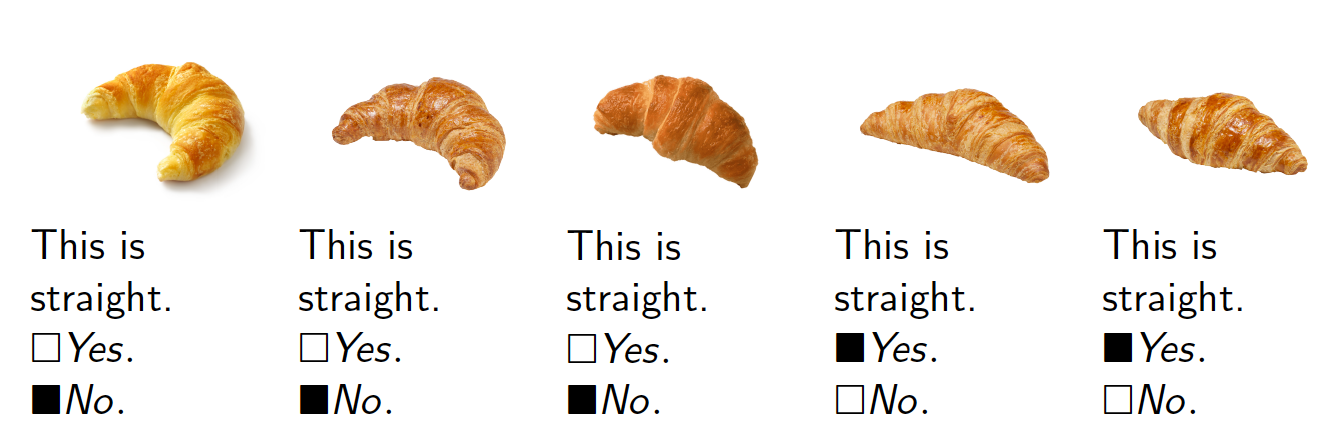
\includegraphics[width=8cm]{images/this-is_straight_croissant.png}
\\
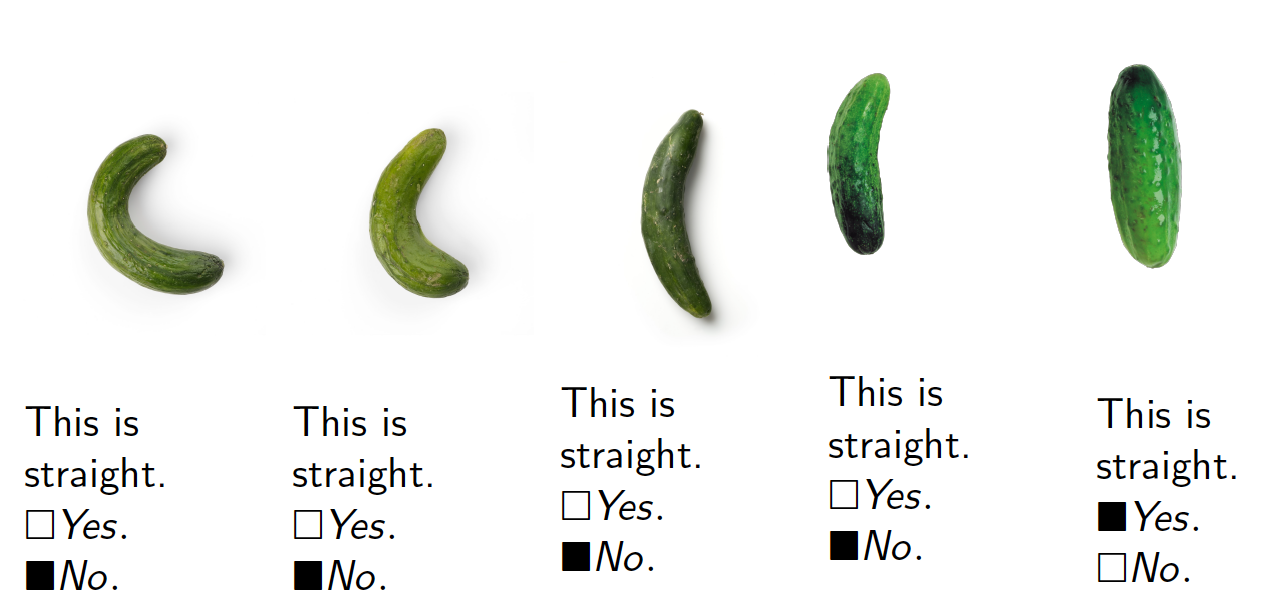
\includegraphics[width=8cm]{images/this-is_straight_cucumber.png}
\\
\\
\textcolor{OliveGreen}{Minimum standard}\\
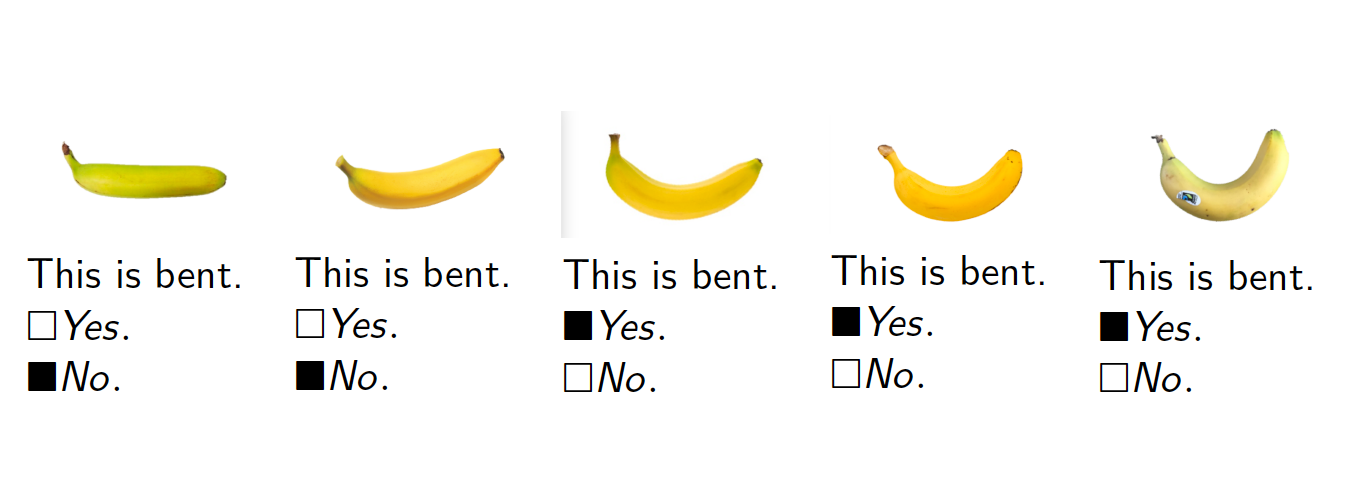
\includegraphics[width=8cm]{images/this_is-bent_banana.png}
\\
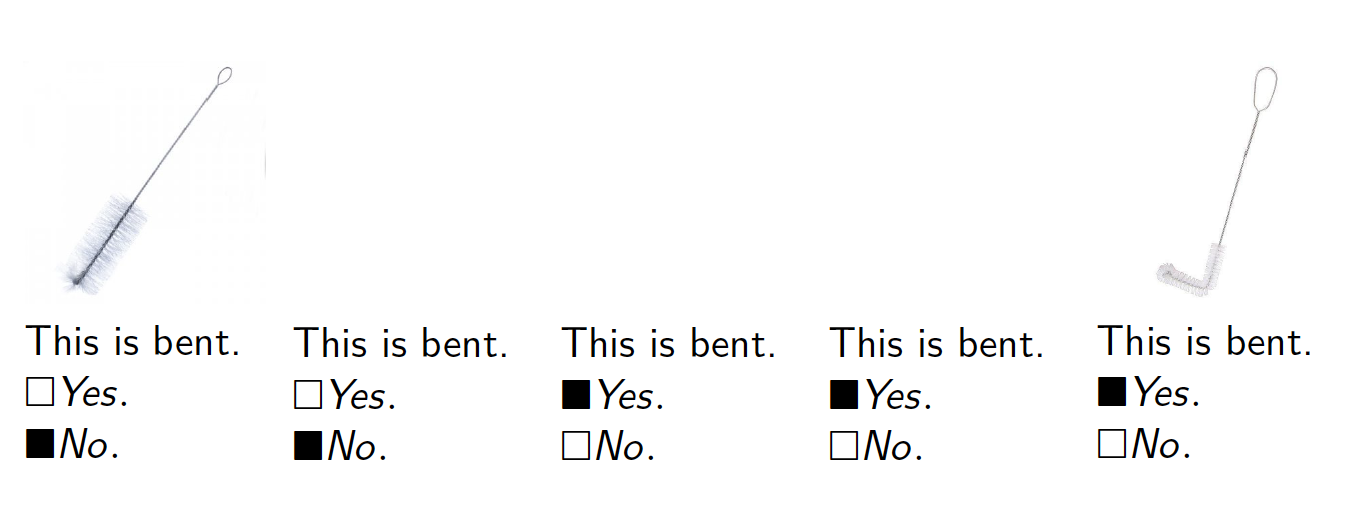
\includegraphics[width=8cm]{images/this_is-bent_brush.png}
\\
\\
\textbf{Relative Adjectives}
World knowledge allows for using scale position 1 as the threshold, e.g. a 'high bed' is already high {\small(sorry! the pics here are not to scale!)}. Hypothetical judgments:\\
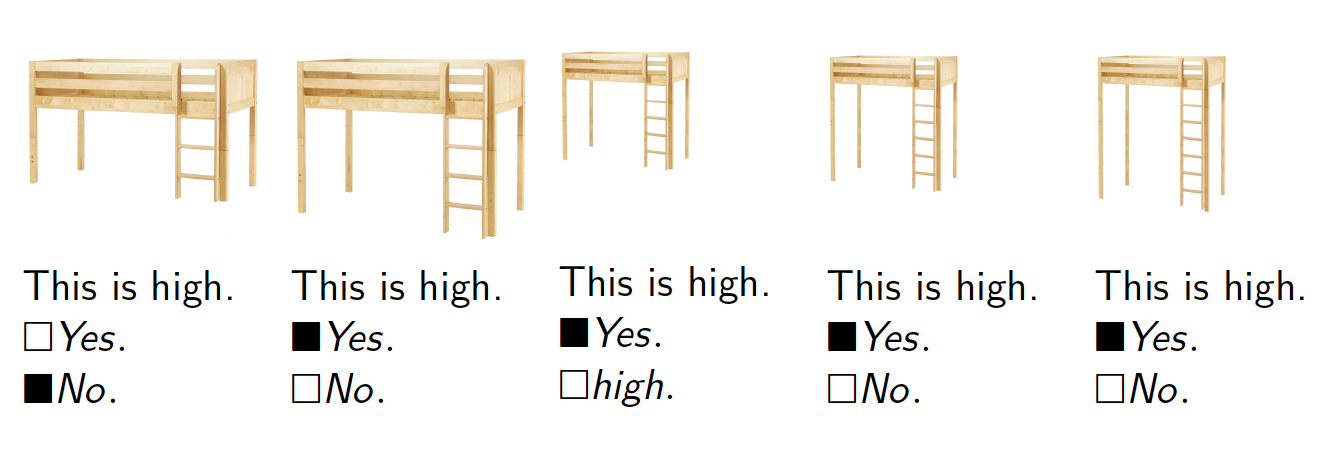
\includegraphics[width=8cm]{images/this_is-high-bed.png}
\\
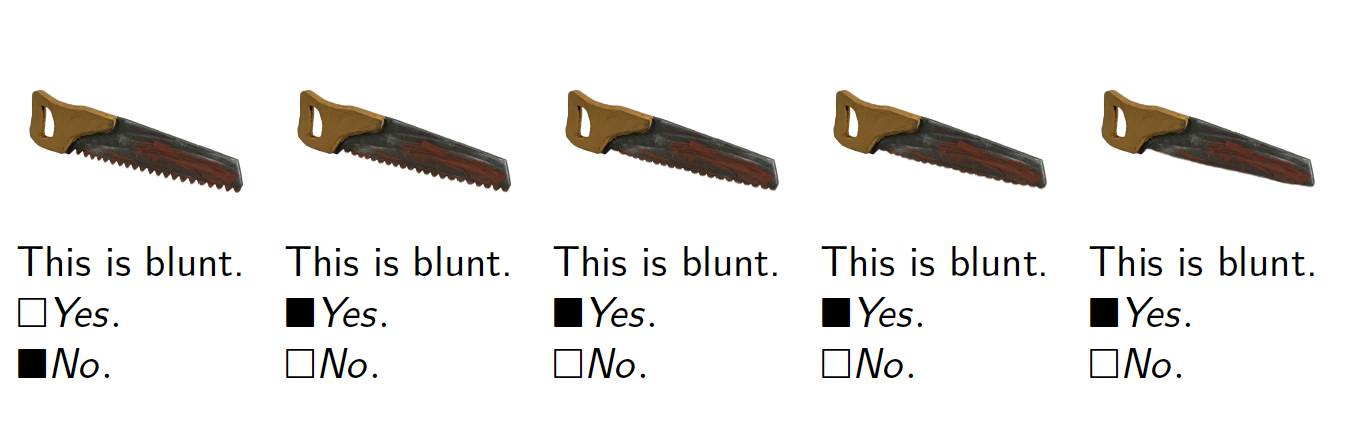
\includegraphics[width=8cm]{images/this_is-blunt_saw.png}
\\
\\
\textbf{Hypothetical results}\\
\textcolor{blue}{Maximum standard absolute adjectives} should elicit some Yes answers already at scale position 3. Conversely, with \textcolor{OliveGreen}{minimum standard adjectives} we should get No's also at position 2 (see graph below). \\
In the experiments by the Chicago group and others, judgments for \textbf{relative adjectives unfamiliar thresholds} align in the characteristic S-shape - black line in the graph below. That's because the threshold gets set with respect to the five objects in the comparison class: it's above the 'average', i.e. position 3. \textcolor{red}{With familiar comparison classes}, we expect that the distribution will shift and resemble the profile for minimum standard adjectives (see also theoretical arguments in e.g., Burnett ...) \\
\begin{multicols}{2}

\\
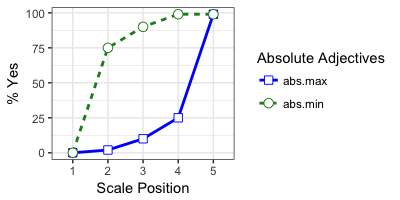
\includegraphics[width=8cm]{images/hypothetical_absolute.png}\\
\\
\columnbreak

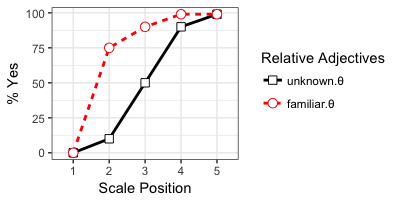
\includegraphics[width=8cm]{images/hypothetical_relative.png}
\end{multicols}

\subsection{Experiment 2 - Reaction Times}
If the ratings profiles for absolute minumum and relative adjectives come out similar, we compare the RTs for the decisions at the corresponding scale positions. \Rightarrow$ Experiment 3: compare ERPs.$


\section{Future music}

Two \textbf{big issues} to ponder:

\begin{itemize}
\item how to derive predictions about response reaction times from prob-models?
\item how to link model predictions to data from some suitable EEG study?
\end{itemize}





% \begin{alignat*}{6}
%   & P_{LL}(t \mid m, \red{l}) && = P(t \mid \den{m}^{\red{l}}) \ \ \propto \ \ P(t) \ \delta_{t
%     \in \den{m}^{\red{l}}}  \\
%   & P_{S_1}(m \mid t \, , \red{l} \, ; \, \lambda_1) && \propto \expo(\lambda_1 \cdot \log
%   P_{LL}(t \mid m , \red{l})  \\
%   & P_{L_1}(t, \red{l} \mid m \, ; \, \lambda_1) && \propto P(t) \cdot P(\red{l}) \cdot P_{S_1}(m
%   \mid t \, , \red{l} \, ; \, \lambda_1) \\
%   & P_{L_1}(t  \mid m \, ; \, \lambda_1)  &&  = \sum_{l} P_{L_1}(t, \red{l} \mid m \, ; \, \lambda_1) \\
%   & P_{S_2}(m \mid t \, ; \, \lambda_1 \, , \lambda_2) && \propto \expo(\lambda_2 \cdot \log P_{L_1}(t
%   \mid m \, ; \, \lambda_1)) \\
%   & P_{L_2}(t  \mid m \, ; \, \lambda_1 \, , \lambda_2) && \propto P(t) \cdot P_{S_2}(m
%   \mid t \, ; \, \lambda_1 \, , \lambda_2)
% \end{alignat*}

\printbibliography[heading=bibintoc]

\end{document}












